\subsection{Raspberry Pi Daten anzeigen}
\label{subsec:DatenAnzeigen}
In dieser Sektion soll die Logik implementiert werden, um die Daten vom Raspberry Pi auf der
Benutzeroberfläche anzuzeigen. Dafür wird ein
\emph{Timer} implementiert, der die Daten liest
\newline
\newline
Damit etwas auf der Benutzeroberfläche angezeigt werden kann, muss das \emph{HTML-Markup}
implementiert werden:

\begin{lstlisting}[language={[Sharp]C}, caption=HTML-Markup,
    label=lst:HtmlMarkup]
<div class="divHeader">
    <div>
        <h1>Raspberry Pi</h1>

        <h2>Uhrzeit: @_uhrzeit</h2>
    </div>

    <div>
        <h3>Temperature Sensor 1: @_temperatur</h3>
        <h3>Temperature Sensor 2: @_temperatur2</h3>
        <h3>Luftdruck: @_pressure</h3>
        <h3>Luftfeuchtigkeit: @_humidity</h3>
    </div>
</div>
\end{lstlisting}

Dabei signalisiert das \emph{@<name>}, dass es sich dabei um eine Variable handelt, die im Code
deklariert wurde.
\newline
\newline
Weitergehend bietet Blazor verschiedene \emph{Render-Funktionen} die nach bestimmten Ereignissen
aufgerufen werden. Wie zum Beispiel die \emph{OnInitializedAsync}, die aufgerufen wird, sobald die
Komponente geladen wird. Diese \emph{OnInitializedAsync} kann nun dazu genutzt werden, um die
Variablen zu initialisieren.

\begin{lstlisting}[language={[Sharp]C}, caption=Render-Funktion: OnInitializedAsync,
    label=lst:OnInitializedAsync]
    protected override Task OnInitializedAsync()
    {
        _senseHat = new();
        _cultureInfo = new("de-DE");
        _uhrzeit = DateTime.Now.ToString("HH:mm:ss", _cultureInfo);

        _temperatur = string.Empty;
        _temperatur2 = string.Empty;
        _pressure = string.Empty;
        _humidity = string.Empty;

        return base.OnInitializedAsync();
    }
\end{lstlisting}

Es soll zudem eine Hilfsfunktion \emph{SetRaspValues} geschaffen werden, die die Daten
ausliest. Diese Funktion wird dann auch in der \emph{OnInitializedAsync} Funktion aufgerufen.

\begin{lstlisting}[language={[Sharp]C}, caption=Funktion: SetRaspValues,
    label=lst:SetRaspValues]
    private void SetRaspValues()
    {
        _temperatur = $"{_senseHat.Temperature.DegreesCelsius:0.#}\u00B0C";
        _temperatur2 = $"{_senseHat.Temperature2.DegreesCelsius:0.#}\u00B0C";
        _pressure = $"{_senseHat.Pressure.Hectopascals:0.##} hPa";
        _humidity = $"{_senseHat.Humidity.Percent:0.#}%";
    }
\end{lstlisting}

Die Hilfsfunktion kann dann in einem Timer genutzt werden. Dieser Timer soll jede Sekunde
aufgerufen werden, um die Werte zu aktualliesieren.

\begin{lstlisting}[language={[Sharp]C}, caption=Timer: ReadTimer,
    label=lst:ReadTimer]
    private void StartTimer()
    {
        _readTimer = new(1000);
        _readTimer.Elapsed += GetData;
        _readTimer.Enabled = true;
    }

    private void GetData(Object source, System.Timers.ElapsedEventArgs e)
    {
        _uhrzeit = DateTime.Now.ToString("HH:mm:ss", cultureInfo);
        SetRaspValues();
        InvokeAsync(StateHasChanged);
    }
\end{lstlisting}

Da die Werte in einem Timer aktuallisiert werden, kann \emph{Blazor} die Änderungen nicht
automatisch feststellen. Dieses Verhalten kommt dadurch, da der Timer nicht auf dem
\emph{Ui-Thread} läuft. Um \emph{Blazor} zu signalisieren, dass Änderungen
vorhanden sind, kann manuell die Funktion \emph{StateHasChanged} aufgerufen werden. Diese
Funktion löst einen neuen \emph{Render-Vorgang} aus.
\newline
\newline
Der momentane Stand der Seite zieht so aus:

\begin{figure}[h]
    \centering
    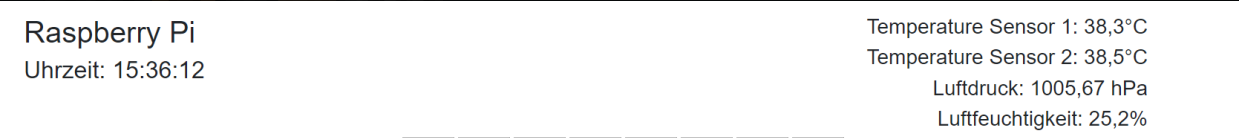
\includegraphics[width=\textwidth, center]{BlazorRasp/BlazorDatenAnzeigen}
    \caption[Zwischenstand der Blazor Demo]{Zwischenstand der Blazor Demo}
    \label{img:BlazorDatenAnzeigen}
\end{figure}